\section{Parallel Processing}

Many stages of a radar signal processing pipeline — range compression, coherent 
integration, CFAR, and angle estimation — involve applying the same operation 
independently across large volumes of data. CPUs, GPUs, FPGAs, and ASICs each offer 
different trade-offs between flexibility, throughput, power efficiency, and development 
effort.

\begin{figure}
    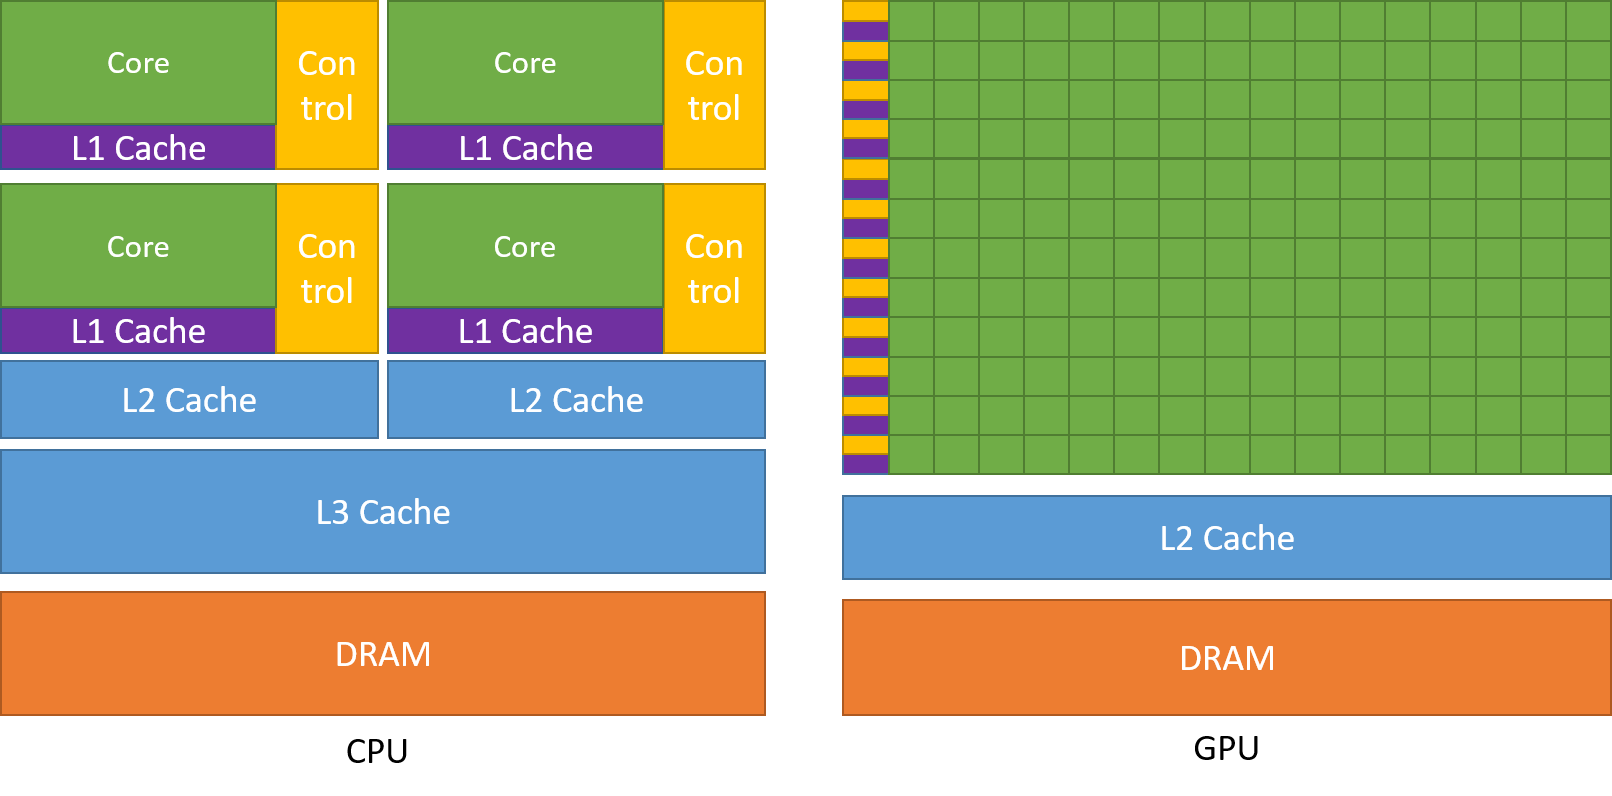
\includegraphics[width=0.8\linewidth]{Images/gpu-devotes-more-transistors-to-data-processing.png}
    \caption[GPU vs CPU transistor allocation for data processing.]{The GPU devotes 
more transistors to data processing than the CPU. Each (green) core acts as a thread 
that executes the same instruction on different data elements. Source: 
\cite{nvidia2025cuda}.}
    \label{fig:gpu-architecture}
\end{figure}        

A GPU executes a large number of lightweight threads (Figure 
\ref{fig:gpu-architecture}), organised into warps, groups of 32 threads that execute 
the same instruction simultaneously on a single streaming multiprocessor (SM). This 
single-instruction multiple-thread (SIMT) model maps directly onto operations such as 
FFTs, element-wise multiplication, and threshold comparisons, where the same 
computation is applied independently to many data elements. When threads within a warp 
follow different control flow paths — a condition known as warp divergence — the 
divergent branches must be executed serially, reducing parallelism (see Figure 
\ref{fig:warp-diverge}).

\begin{figure}
    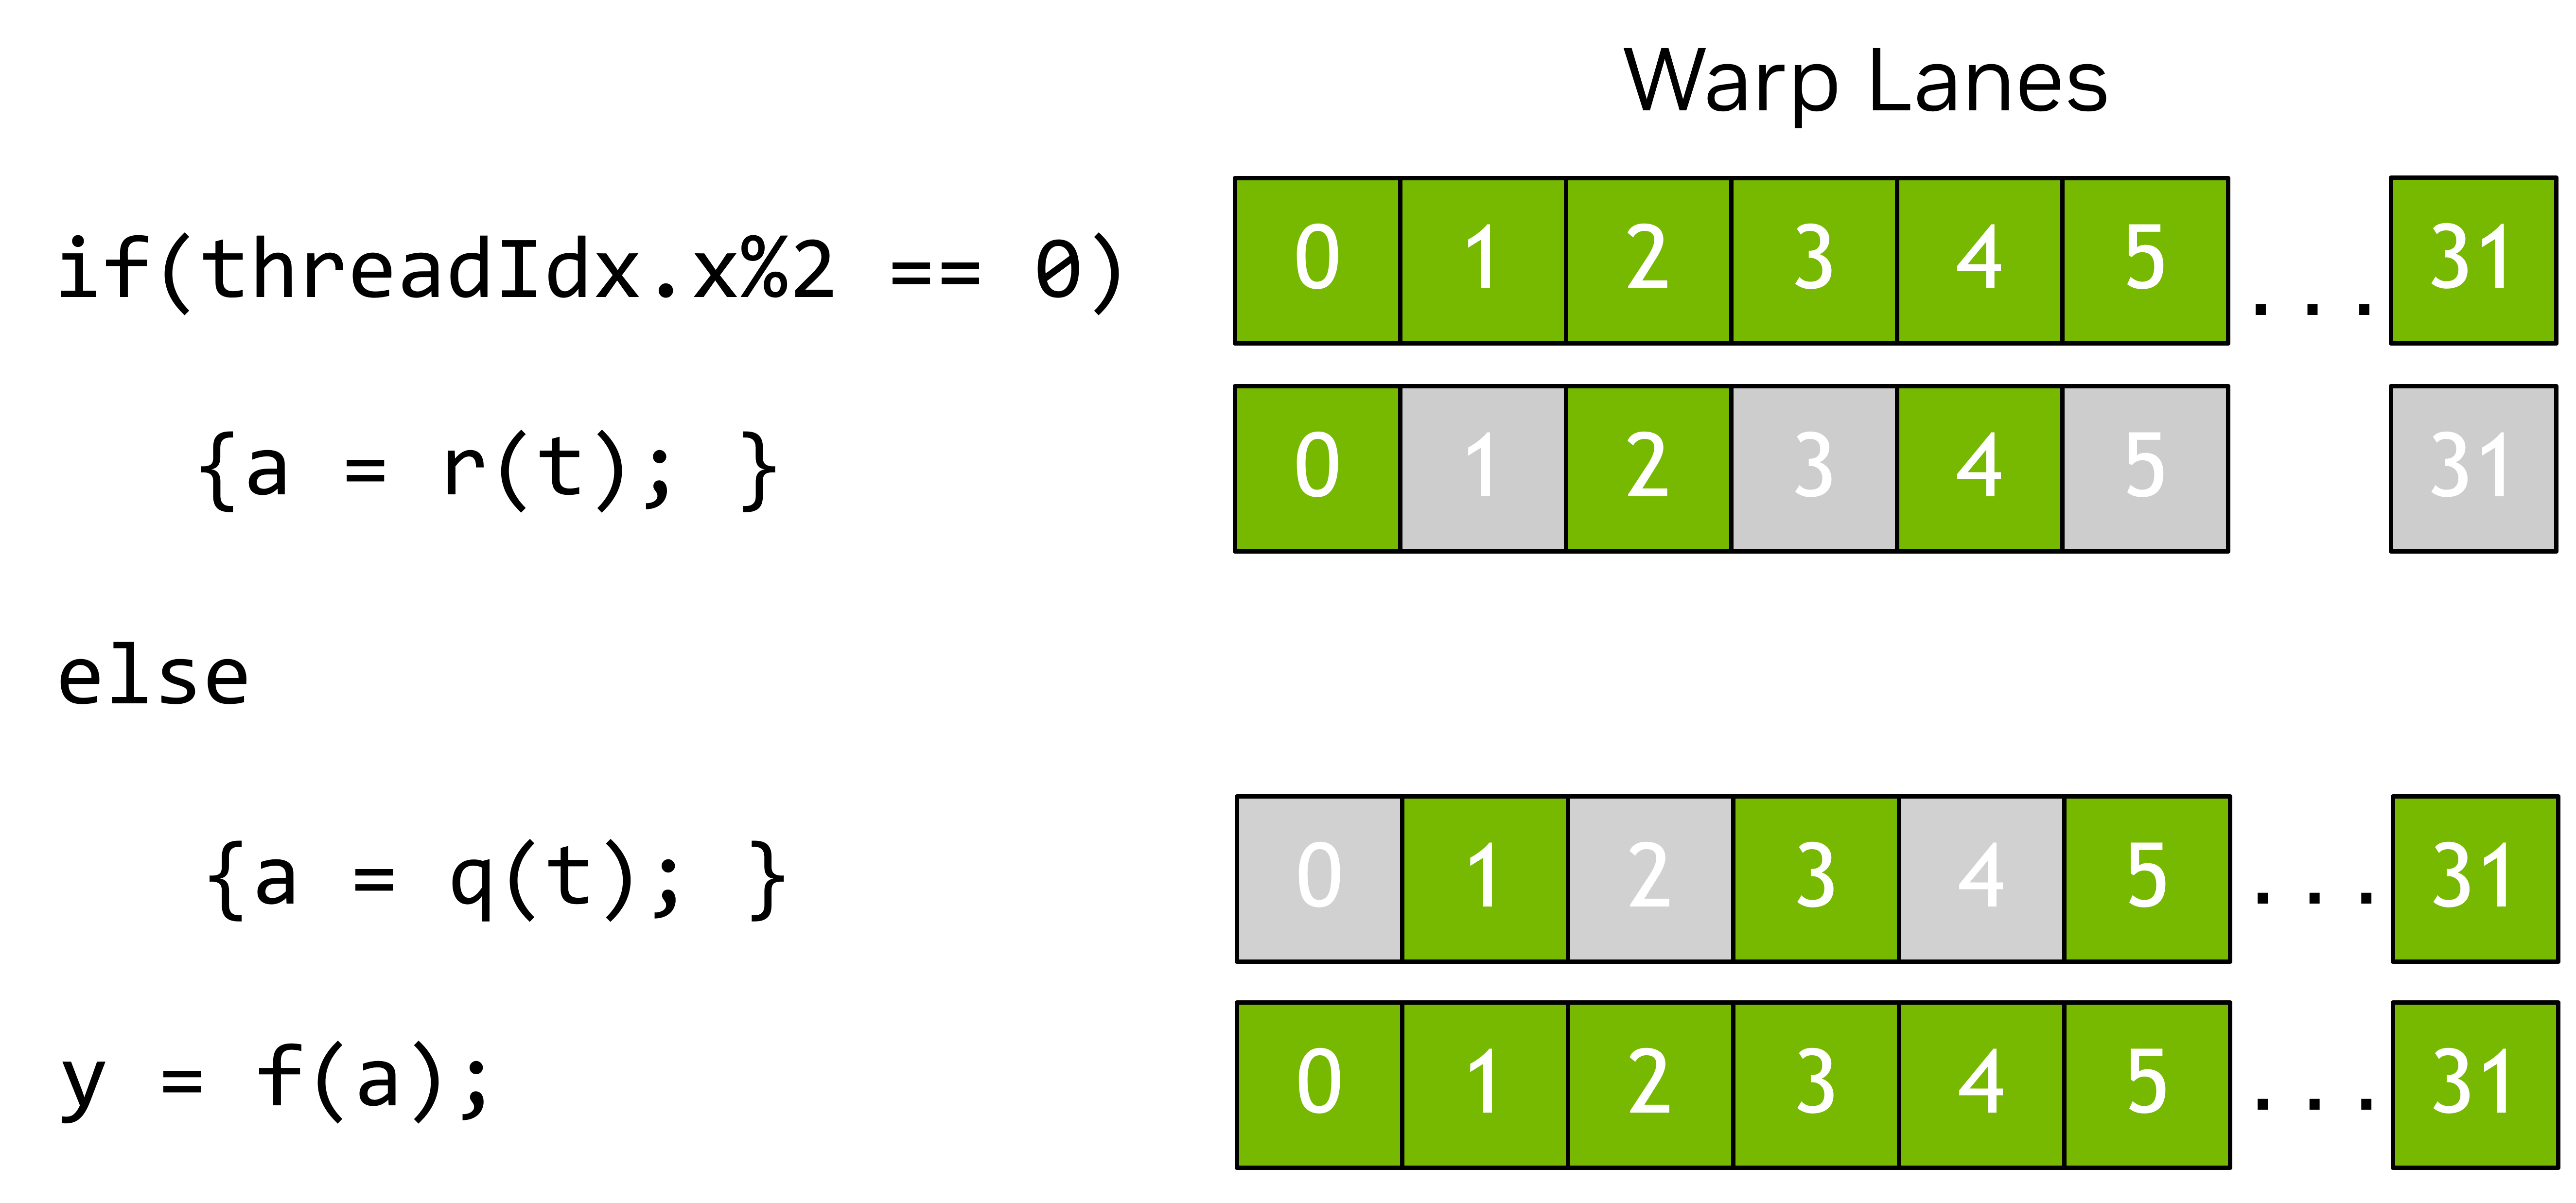
\includegraphics[width=0.8\linewidth]{Images/active-warp-lanes.png}
    \caption[Warp divergence causing serial execution of divergent branches.]{In this example, branching
    paths in execution between the even and odd threads prevent all threads from executing in parallel.
    All even threads execute the top branch while all odd threads are idle, then vice versa. As a result,
    the execution time is the sum of the two branches instead of the maximum. 
    Source: \cite{nvidia2025cuda}.}
    \label{fig:warp-diverge}
\end{figure}

Memory access patterns also affect throughput. Global memory is accessed most 
efficiently when threads in a warp read or write contiguous memory locations 
simultaneously, a pattern known as coalesced access. Non-coalesced access wastes
memory bandwidth by reading non-contiguous memory locations.
Figure \ref{fig:coalesced-access} illustrates one such situation. The warps will need 
to retrieve data from global memory more frequently when accessing non-contiguous 
memory. For this reason, ensuring that as much as possible of the data in each cache 
line fetched is actually used is an important part of performance optimisation of 
memory accesses on these devices.

\begin{figure}
    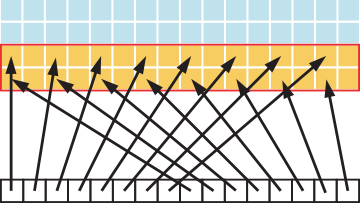
\includegraphics[width=0.5\linewidth]{Images/adjacent-threads-accessing-memory-with-stride-of-2.png}
    \caption[Non-coalesced memory access with stride of 2 reducing bandwidth efficiency.]{Figure 6:
    Adjacent threads (bottom) accessing every second memory location (orange). Since memory is cached in 
    large blocks,
    the large stride of 2 results in a 50\% reduction in load/store efficiency, since half of all cached
    memory is not being used. Source: \cite{nvidia2025cuda}.}
    \label{fig:coalesced-access}
\end{figure}

In discrete GPU systems, the CPU and GPU maintain separate physical memory pools 
connected by a bus such as PCIe, and data must be explicitly transferred between host 
and device memory. In system-on-chip (SoC) platforms such as the NVIDIA Jetson family, 
the CPU and GPU share the same physical DRAM. This is called physically shared memory. 
Both processors access the same physical addresses, and the memory subsystem handles 
coherency, eliminating the explicit transfer step.

Shared memory is a separate, small, low-latency scratchpad memory local to each SM, 
explicitly managed by the programmer. It allows threads within a thread block to 
exchange data and cache intermediate results without accessing global memory. It is 
used in GPU implementations of reductions, transpose operations, and tiled matrix 
multiplications, where threads cooperatively load a tile of data into shared memory and 
reuse it across multiple operations.